\begin{algorithm}[H]
    \SetAlgoLined
    \SetKwInOut{Input}{Input}
    \SetKwInOut{Output}{Output}
    \Input{\texttt{TestPoint $\mathcal{T}(\boldsymbol{x}, \boldsymbol{y}) ; [x \in \mathbb{R};y \in \mathbb{R}]$, $dim$; $2$, $split\_axis$ ($\mathcal{S}$) ; $0/1$ ($0$; $x\_axis$ and $1$; $y\_axis$)}}
    \Output{\texttt{Value associated with $\mathcal{T}(\boldsymbol{x}, \boldsymbol{y})$}}
    \texttt{SEARCH\_POINT\_QUERY($dim$, $\mathcal{S}$)}\\
    \texttt{Start at root}\\
    \eIf {node is leaf}
        {
            \texttt{return value associated with node}
        }
        {
        \eIf{\texttt{$\mathcal{T}(\boldsymbol{x}, \boldsymbol{y})$ $\mathcal{S}$ value > node $\mathcal{S}$ value}}
            {\texttt{Traverse to node.rightChild}\\ \texttt{SEARCH\_POINT\_QUERY($dim$, $(\mathcal{S}+1) \% dim$)}}
        {\texttt{Traverse to node.leftChild}\\ 
        \texttt{SEARCH\_POINT\_QUERY($dim$, $(\mathcal{S}+1) \% dim$)}}
        }
    \caption{Point Query Algorithm for $K$D-Tree}
    \label{Point_Query_Algorithm_$K$D-Tree}
\end{algorithm}

In algorithm \ref{Point_Query_Algorithm_$K$D-Tree} 

\begin{enumerate}

    \item On line $2$, start traversing the tree from the root. 
    
    \item On line $3$, check if the point is a leaf. If it is a leaf then we can simply return the value associated with the point.
    
    \item On line $5$, if root point is not a leaf then we make a decision whether to go left or right.
    
    \item On line $6$, we make this decision based on $\mathcal{S}$ value associated with the point. At the root, we start with $\mathcal{S}$ as $0$ ($x\_axis$). 
    \item On line $8$ and $11$, we then recursively call the function SEARCH\_POINT\_QUERY() and update the $\mathcal{S}$ between $0$ and $1$ alternatively as we increase levels until we reach a leaf.

\end{enumerate}

\begin{mscexample}
    \begin{minipage}[t]{\linewidth}
        \centering
        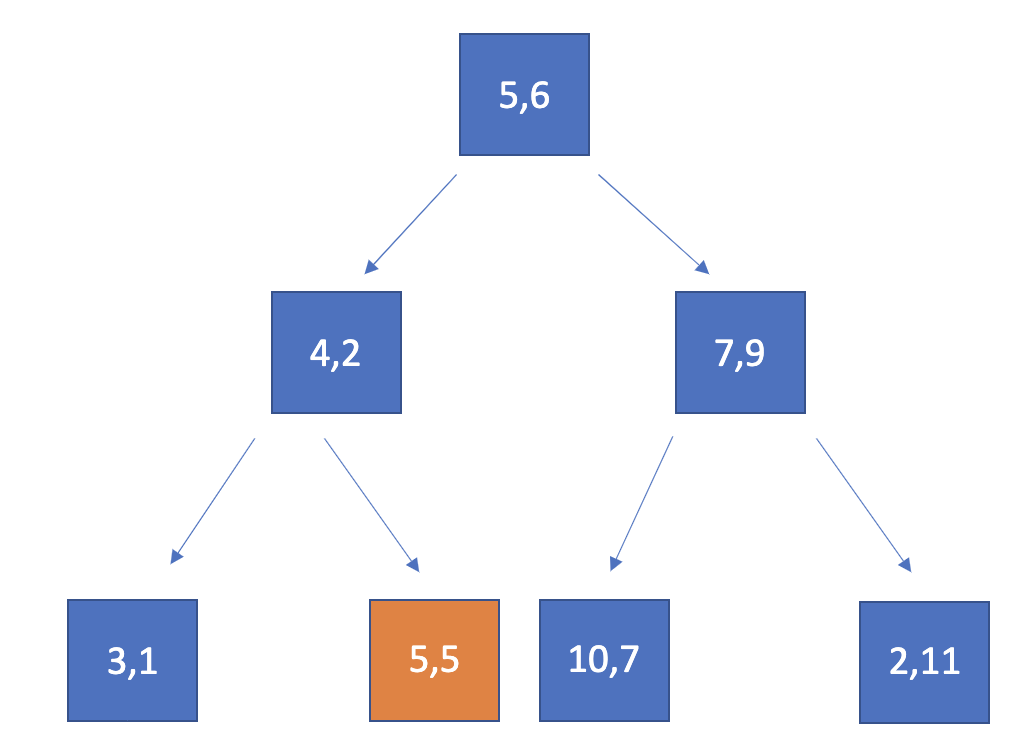
\includegraphics[width=7cm]{graphs/KD_Tree_Point_Query_Tree.png}
        % \caption{$K$D-Tree for Point Query (TestPoint $\mathcal{T}(\boldsymbol{x}, \boldsymbol{y})$ = $(5,5)$ is highlighted in orange)}
        \label{fig:$K$D-Tree_for_Point Query}
    \end{minipage}
    
    \textbf{Case 1} : For example we have a tree with Point list as 
	$$[(5,6),(4,2),(7,9),(3,1),(5,5),(10,7),(2,11)]$$
    Suppose we are looking for $\mathcal{T}(\boldsymbol{x}, \boldsymbol{y})$ = $(5,5)$.
    Below are the steps we follow in order to search the point:
    \begin{enumerate}
         \item We start with root point $(5,6)$ and $\mathcal{S}$ as $0$. 
         
         \item Since $\mathcal{S}$ is $0$, we compare the $x\_axis$ of the $\mathcal{T}(\boldsymbol{x}, \boldsymbol{y})$ and root point. Since they are equal($5 = 5$), we move left of the root node. 
         
         \item Increase $\mathcal{S}$ to $1$. 
         
         \item Compare the $y\_axis$ of point $(4,2)$ and  $\mathcal{T}(\boldsymbol{x}, \boldsymbol{y})$. Since $5 > 2$, we move to the right of the tree. 
         
         \item Since node $(5,5)$ is a leaf, we return the value associated with the point. 
    \end{enumerate}
\end{mscexample}
